\section{Preliminaries}\label{sec:prelim}
We begin with some background that we need to describe the concept of inconsistency measures for private databases. 

\def\tids{\mathit{tids}}

\subsection{Database and Constraints}\label{sec:prelim-integrity-constraints}
We consider a single-relation schema $\attrset = (A_1, \ldots, A_m)$, which is a vector of distinct attribute names $A_i$, each associated with a domain $\dom(A_i)$ of values. A database $D$ over $\attrset$ is a associated with a set $\tids(D)$ of \emph{tuple identifiers}, and it maps every identifier $i\in\tids(D)$ to a tuple $D[i]=(a_1,\dots,a_m)$ in $A_1\times\dots\times A_m$. A database $D'$ is a \emph{subset} of $D$, denoted $D'\subseteq D$, if  $D'$ is obtained from $D$ by deleting zero or more tuples, that is, $\tids(D')\subseteq\tids(D)$ and $D'[i]=D[i]$ for all $i\in\tids(D')$.

Following previous work on related topics~\cite{DBLP:journals/pvldb/GeMHI21,DBLP:journals/pvldb/LivshitsHIK20}, we focus on Denial Constraints (DCs) on pairs of tuples. Using the formalism of Tuple Relational Calculus, such a DC is of the form
$\forall t,t' \neg \big(\varphi_1\land\dots\land\varphi_k\big)$ where each $\varphi_j$ is a comparison $\sigma_1\circ\sigma_2$ so that: (a) each of $\sigma_1$ and $\sigma_2$ is either $t[A_i]$, or $t'[A_i]$, or $a$, where $A_i$ is some attribute and $a$ is a constant value, and (b) the operator $\circ$ belongs to set $\{<, >, \leq, \geq, =, \neq\}$ of comparisons. This DC states that there cannot be two tuples $t$ and $t'$ such that all comparisons $\varphi_j$ hold true (i.e., at least one $\varphi_j$ should be violated).

Note that the class of DCs of the form that we consider generalizes the class of Functional Dependencies (FDs). An FD has the form $X\rightarrow Y$ where $X,Y\subseteq\{A_1,\dots,A_m\}$, and it states that every two tuples that agree on (i.e., have the same value in each attribute of) $X$ must also agree on $Y$.

In the remainder of the paper, we denote by $\constraintset$ the given set of DCs. A database $D$ \emph{satisfies} $\constraintset$, denoted $D \models \constraintset$, if $D$
satisfies every DC in $\constraintset$; otherwise, $D$ \emph{violates} $\constraintset$, denoted $D \not\models \constraintset$.

%, and $D$ is a bag of $n$ tuples such that $\dom(D) = \dom(A_1) \times \ldots \times \dom(A_m)$. That is, each element of $D$ is a tuple $t = (a_1, \ldots, a_m)$, where $a_i \in \dom(A_i)$. 


%xh{I agree with Benny for the notation issues. Please check the preliminaries in Benny's paper \cite{LivshitsKTIKR21}.}

%In this work, we consider a single-table database $D$ over a schema $\attrset = (A_1, \ldots, A_m)$, where each $A_i$ is an attribute name and $\attrset$ is a vector of attribute names, and $D$ is a bag of $n$ tuples such that $\dom(D) = \dom(A_1) \times \ldots \times \dom(A_m)$. That is, each element of $D$ is a tuple $t = (a_1, \ldots, a_m)$, where $a_i \in \dom(A_i)$. 

% A Functional Dependency (FD) is a statement of the form $X \rightarrow Y$, where $X, Y \subseteq \attrset$, stating that every two tuples that have the same values for the all the attributes in $X$ should also have the same values for all attributes in $Y$. 
%A Denial Constraint (DC) can be expressed as a first-order formula in the form $ \sigma : \forall t_i, t_j \in D, \neg(\phi_1 \land \ldots \land \phi_k)$. Each $\phi_i$ is of the form $a_1 \circ a_2$ or $a_1 \circ c$ where $a_1, a_2 \in t_x[A], x \in \{i, j, \dots, \}, A \in \attrset$,  $\circ \in \{<, >, \leq, \geq, =, \neq\}$, and $c$ is a constant.\benny{ Several issues. First, I cannot understand the definition. What does "$a_1, a_2 \in t_x[A]$" mean exactly? Second, it is bad style to write math-comma-math (since the expressions might be ambiguous... which comma is text and which comma is math?). Third, a DC cannot be expressed in the way you write, generally. Only after this sentence, you are saying that we look at binary DCs... Fourth, $\forall t_i, t_j$ is TRC, not FO. In FO you can quantify only on variables... here ou quantify on tuples and you have this special t[A] expressions... this is allowed in TRC, not in FO (DRC). }
 %In this paper, we consider only binary DCs (i.e. predicates in $\sigma$ are over 2 tuples). 
%\sm{room for improvement here with k-ary DCs.}
%A DC states that a pair of tuples cannot satisfy all predicates $\phi_i$ included in it. A functional dependency (FD), $A \rightarrow B$ where $A = \{\phi_1 \land \ldots \land \phi_k\}$ and $B = \{\psi\}$, \benny{This is not conventional for FDs. First, in FDs, $A$ and $B$ (capitals from the beginning of the alphabet) denote single attributes. An FD is written as $X\rightarrow Y$, where $X$ and $Y$ are sets of attributes. What are the $\phi_i$? What is $\psi_i$? Are these predicates (as in the case of a DC)?}
%can be written as a DC as follows: $ \sigma : \forall t_i, t_j \dots \in D, \neg(\phi_1 \land \ldots \land \phi_k \land \psi)$ where $\phi_i$ is an equality predicate ($=$) and $\psi$ is a inequality ($\neq$) formula. 
% A DC is also said to be anti-monotonic if the consistency cannot be violated by deleting tuples. For example, a functional dependency is anti-monotonic. 


\def\set#1{\mathord{\{#1\}}}
A common way of capturing the violations of $\constraintset$ in $D$ is through the \emph{conflict graph} $\graph$, which is the graph $(V, E)$, where $V=\tids(D)$ an edge $e = \set{i,j} \in E$ occurs whenever the tuples $D[i]$ and jointly $D[j]$ violate $\constraintset$. 
%\benny{We never said that tuples have tuple identifiers... this is not in our formal model.} 
To simplify the notation, we may write simply $\mathcal{G}$ instead of $\graph$ when there is no risk of ambiguity.
%We note that there might be multiple edges between two tuples $i$ and $j$ due to multiple violations but we consider only one of them. 
% We also remove self edges where the tuple violates and itself for our work. 
%\xh{May refer to the example in Figure~\ref{fig:db_to_graph} here instead of the algorithm part}

\begin{example}
     Consider a dataset that stores information about capital and country as shown in Figure~\ref{fig:db_to_graph}. Assume an FD constraint $\sigma: \mbox{Capital} \rightarrow \mbox{Country}$ between attributes capital and country that says that the country of two tuples must be the same if their capital is the same. Assume the dataset has 3 rows (white color) and a neighboring dataset has an extra row (grey color) with the typo in its country attribute. As shown in the right side of Figure~\ref{fig:db_to_graph}, the dataset with 4 rows can be converted to a conflict graph with the nodes corresponding to each tuple and edges referring to conflicts between them. The $\mininconsistency$ measure computes the size of the set of all minimally inconsistent subsets $|MI_\constraintset(D)|$ (the number of edges in the graph) for this dataset. %has a sensitivity equal to the size of the dataset (in this case, 3) as adding a violating row violates all other rows. \sm{notion of sensitivity is not introduced yet. is that okay? }
     \label{example:running_example}
\end{example}

\begin{figure}
%\small
    \centering
    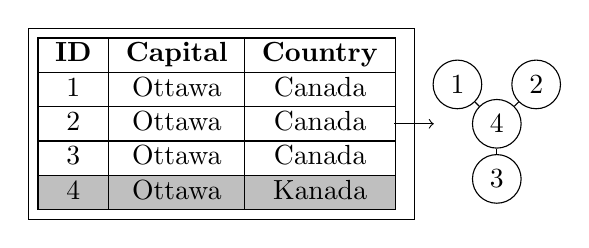
\begin{tikzpicture}
    % Define the table
    \node[draw, align=center] (table) at (1.5,0) {
        \begin{tabular}{|c|c|c|}
            \hline
            \textbf{ID} & \textbf{Capital} & \textbf{Country} \\
            \hline
            1 & Ottawa & Canada \\
            \hline
            2 & Ottawa & Canada \\
            \hline
            3 & Ottawa & Canada \\
            \hline
             \rowcolor{lightgray}
            4 & Ottawa & Kanada \\
            \hline
        \end{tabular}
    };

    % Define the graph
    
    \node[draw, circle] (node1) at (4.5,0.5) {1};
    \node[draw, circle] (node2) at (5.5,0.5) {2};
    \node[draw, circle] (node3) at (5,-0.7) {3};
    \node[draw, circle] (node4) at (5,0) {4};
    \draw (node1) -- (node4);
    \draw (node2) -- (node4);
    \draw (node3) -- (node4);
    
    % Draw the arrow
    % \draw[->] (table.east) -- (node4.west);
    \draw[->] (3.7, 0) -- (4.2, 0);
\end{tikzpicture}
   \vspace{0.2cm} % Add space below the figure
    % \includegraphics[width=\linewidth]{images/database_to_graph.jpg}
    \caption{Toy example dataset to show a worst-case analysis. An additional row may violate all other rows in the dataset (left). Easier analysis can be done by instead converting the dataset into its corresponding conflict graph (right).
    }
    \label{fig:db_to_graph}
    % Image link: https://docs.google.com/drawings/d/1ibadfqHlWPfEwiOApukretrSKzGyi9w6-pv5OX8Y3sI/edit?usp=sharing
\end{figure}

%
\begin{lstlisting}[breaklines=true, caption={Qualitative Example 5: An example trace in the summarization domain, with \reactagent{} when using \texttt{gpt-4-turbo} as LLM.},label={ls:qualsummary}]
# Alice Anastasiou says: I'm interested in compiling a summary on the topic: governor, race, gop, obamacare, medicaid. Can you help me? 
>>>  Reflection.thought("I will first resolve the primary user to get the right contact information")
>>>  Enterprise.resolve_primary_user()
{"email": "alice@company.com", "full_name": "Alice Anastasiou", "user_id": "alice"}
>>>  Reflection.thought("I will search user's documents and find relevant people who may have more information")
>>>  EnterpriseSearch.search_documents(query="governor, race, gop, obamacare, medicaid")
>>>  EnterpriseSearch.search_relevant_people(query="governor, race, gop, obamacare, medicaid")
{"parker": "Knows about the following topics:\ngovernor elections, GOP, health care, Obama, Romney", "bhushan": "Knows about the following topics:\ngovernor elections, GOP, health care, Obama, Romney\nSiskiyou County, California, secession, state of Jefferson, rural representation", "farshid": "Knows about the following topics:\nSiskiyou County, secession, Jefferson, California, rural fire prevention fee", "eden": "Knows about the following topics:\nFacebook, gay rights, John Snow kiss-in, Richard Metzger, Paul Shetler\nFacebook, same-sex kissing, photo removal, protest", "hannah": "Knows about the following topics:\n", "dewei": "Knows about the following topics:\n", "cassie": "Knows about the following topics:\n"}
>>>  Reflection.thought("Parker and Bhushan have information about the governor race and GOP, so I should reach out to them.")
>>>  Enterprise.send_message("alice", "Hi Alice, I can reach out to Parker and Bhushan to produce a summary. Is that OK?")
>>>  System.finish()

# Alice Anastasiou says: Yes, please do that. 
>>>  Reflection.thought("I will reach out to Parker to ask for information about the governor race and GOP")
>>>  Enterprise.resolve_person("Parker")
{"email": "parker@company.com", "full_name": "Parker McLean", "user_id": "parker"}
>>>  Enterprise.send_message("parker", "Hi Parker, do you have any information about the governor race, GOP, Obamacare, or Medicaid?", title="Information about governor race and GOP")
>>>  System.finish()

# Parker McLean says: Yes, here's a relevant document I found: "gop eyes gains as voters in 11 states pick governors     enlarge this image toggle caption jim cole/ap jim cole/ap     voters in 11 states will pick their governors tonight , and republicans appear on track to increase [...] "
>>>  Reflection.thought("I will reach out to Bhushan to ask for information about the governor race and GOP")
>>>  Enterprise.resolve_person("Bhushan")
{"email": "bhushan@company.com", "full_name": "Bhushan Magar", "user_id": "bhushan"}
>>>  Enterprise.send_message("bhushan", "Hi Bhushan, do you have any information about the governor race, GOP, Obamacare, or Medicaid?", title="Information about governor race and GOP")
>>>  System.finish()

# Bhushan Magar says: Yes, here's a relevant document I found: "the real clear politics average for the race has mccrory maintaining a 14.3 percentage point lead .     montana : popular democratic gov . brian schweitzer - he won his last election with 65 percent of the vote - has [...]" 
>>>  Reflection.thought("I have enough information to compile the summary. I will send a message to Alice, with the summary enclosed in [[[ brackets ]]].")
>>>  Enterprise.send_message("alice", "Hi Alice, here's the summary I put together: [[[Voters in 11 states are choosing their governors, with Republicans poised to increase their numbers, potentially controlling over two-thirds of the nation's top state offices. The GOP is expected to take North Carolina and retain seats in Utah, North Dakota, and Indiana. Democrats are likely to hold West Virginia and Missouri, with competitive races in Montana, New Hampshire, and Washington. The governor's role is crucial in healthcare, as they can opt out of Medicaid expansion under the Affordable Care Act. A Romney win would empower Republican governors, especially in states where Obama's policies, like high-speed rail funding, were previously rejected.]]]", title="Governor race and GOP summary")

# Alice Anastasiou says: Thank you, this is exactly what I needed. 
>>>  Reflection.thought("Alice has confirmed that no more information is needed. I will close the session")
>>>  Enterprise.send_session_completed()
>>>  System.finish()
\end{lstlisting}




\subsection{Inconsistency Measures}\label{sec:prelim-inconsistency}

\def\MI{\mathord{\mathsf{MI}}}
\def\MC{\mathord{\mathsf{MC}}}


Inconsistency measures have been studied in previous work~\cite{DBLP:conf/sum/Bertossi18,DBLP:conf/ecsqaru/GrantH13,DBLP:journals/ijar/GrantH23,LivshitsK22,LivshitsBKS20} as a means of measuring database quality for a set of DCs. 
We adopt the measures and notation of \citet{LivshitsKTIKR21}. Specifically, they consider five inconsistency measures that capture different aspects of the dataset quality. To define these concepts, we need some notation. Given a database $D$ and a set $\constraintset$ of anti-monotonic integrity constraints, we denote by $\MI_\constraintset(D)$ the set of all \emph{minimally inconsistent subsets}, that is, the sets $E \subseteq D$ such that $E \not\models \constraintset$ but $E' \models \constraintset$ for all $E' \subsetneq E$. We also denote by $\MC_\constraintset(D)$ the set of all \emph{maximal consistent subsets} of $D$; that is, the sets $E \subseteq D$ such that $E \models \constraintset$ and $E' \not\models \constraintset$ whenever $E \subsetneq E' \subseteq D$. 


\begin{definition}[Inconsistency measures~\cite{LivshitsKTIKR21}]\label{def:inconsistencymeasure}
Given a database $D$ and a set of DCs $\constraintset$, the inconsistency measures are defined as follows:
\begin{itemize}
    \item Drastic measure: $\drastic(D, \constraintset) = 1$ if $D \models \constraintset$ and 0 otherwise.
    \item Minimal inconsistency measure:  $\mininconsistency(D,\constraintset) = |\MI_\constraintset(D)|$.
    \item Problematic measure: $\problematic(D,\constraintset) = |\cup \MI_\constraintset(D)|$.
    \item Maximal consistency measure: $\maxconsistency(D,\constraintset) = |\MC_\constraintset(D)|$ \footnote{We drop "-1" from the original definition~\cite{LivshitsKTIKR21} for simplicity.}.
    \item Optimal repair measure: $\repair(D,\constraintset) = |D| - |D_R|$, where $|D_R|$ is the largest subset $D_R \subseteq D$ such that $D_R \models \constraintset$.
    % $min\{\kappa(o,D) \mid o \in O, o(D) \models \constraintset\}$, where $o \in O$ is a set of operations permitted by a repair intervention model $\intervention$ (e.g., repair through tuple deletions or tuple updates) and $\kappa$ is a function that assigns a numerical cost to every sequence $o$. 
\end{itemize}
%where $o \in O$ is a set of operations permitted by an repair intervention model $\intervention$ (e.g., repair through tuple deletions or tuple updates) and $\kappa$ is a function that assigns a numerical cost to every sequence $o$.
\end{definition}

% For simplicity in our work, we consider unit cost for repair function $\kappa$ in the intervention model $\intervention$. 

Observe that inconsistency measures also have a graphical interpretation for the conflict graph \graph. For instance, the drastic measure $\drastic(D,\constraintset)$ corresponds to a binary indicator for whether there exists an edge in $\graph$. We summarize the graph interpretation of these inconsistency measures in Table~\ref{tab:summary}. 


\eat{
We can also define these inconsistency measures in terms of a conflict graph \graph as follows~\cite{LivshitsKTIKR21}: 


\xh{may drop this observation chunk, and points to Table~\ref{tab:summary}}.
\begin{observation}\label{prop:graph-defs}
Given a database $D$, a set of DCs \constraintset, and their corresponding conflict graph \graph, the following holds: 
\begin{enumerate}
    \item $\drastic(D,\constraintset)$ is 1 if there exists at least an edge in \graph, 0 otherwise. 
    \item\label{itm:mininc} $\mininconsistency(D,\constraintset)$ is the number of edges in \graph.
    \item $\problematic(D,\constraintset)$ is the number of nodes in \graph\ that have a positive degree.
    \item $\maxconsistency(D,\constraintset)$ is the number of maximal independent sets in \graph.
    \item $\repair(D,\constraintset)$ is the minimum vertex cover size of \graph. 
\end{enumerate}
\end{observation}
}


\subsection{Differential Privacy}~\label{sec:prelim-dp}
Differential privacy (DP) \cite{dwork2006calibrating} aims to protect private information in the data. In this work, we consider the unbounded DP setting where we define two neighboring datasets, $D$ and $D'$ (denoted by $D \neighbor D'$) if $D'$ can be transformed from $D$ by adding or removing one tuple in $D$.

\def\prob{\mathrm{Pr}}

\begin{definition}[Differential Privacy \cite{dwork2006calibrating}]
    An algorithm $\mathcal{M}$ is said to satisfy $\epsilon$-DP if for all $S\subseteq \mbox{Range}(\mathcal{M})$ and for all $D\neighbor D'$,
        $$\prob[\mathcal{M}(D)\in S] \leq e^\epsilon \prob[\mathcal{M}(D')\in S]\,.$$
\end{definition}

%\benny{Please $\prob[...]$ instead of $Pr[...]$} \benny{Please do not write text in math... for example, use $\mbox{Range}$ instead of $Range$.}


The privacy cost is measured by the parameters $\epsilon$, often called the \emph{privacy budget}. The smaller $\epsilon$ is, the stronger the privacy is.  
Complex DP algorithms can be built from the basic algorithms following two essential properties of differential privacy:

\begin{proposition}[DP Properties~\cite{Dwork06,DworkKMMN06}]\label{prop:DP-comp-post} 
    % \!\emph{\cite{Dwork06,DworkKMMN06}}\, 
    The following hold.
    \begin{enumerate}
        \item {\bf (Sequential composition)} 
        If $\mathcal{M}_i$ satisfies $\epsilon_i$-DP, then the sequential application of $\mathcal{M}_1$, $\mathcal{M}_2, \cdots$,  satisfies $(\sum_{i} \epsilon_i)$-DP.
        
        \item {\bf (Parallel composition)} 
        If each $\mathcal{M}_i$ accesses disjoint sets of tuples, they satisfy $(\max_i \epsilon_i)$-DP together.
        
        \item {\bf (Post-processing)} 
        Any function applied to the output of an $\epsilon$-DP mechanism $\mathcal{M}$ also satisfies $\epsilon$-DP.
    \end{enumerate}
\end{proposition}



Many applications in DP require measuring the change in a particular function's result over two neighboring databases. The supremum over all pairs of neighboring databases is called the \emph{sensitivity} of the function. 

\begin{definition}[Global sensitivity \cite{DworkMNS16}]\label{def:sensitivity}
Given a function $f: \mathcal{D} \rightarrow \mathbb{R}$,  the  sensitivity of $f$ is 
\begin{equation}
\Delta_f = \max\limits_{D'\approx D}|f(D) - f(D')|.
\end{equation}
% $sup_{D' \approx D, D' \subseteq D}{|f(D)-f(D')|}$ and is denoted by $\Delta_f$. 
\end{definition}


\paratitle{Laplace mechanism}
The Laplace mechanism~\cite{DworkMNS16} is a common building block in DP mechanisms and is used to get a noisy estimate for queries with numeric answers. The noise injected is calibrated to the query's global sensitivity.

% \begin{theorem}[Laplace Mechanism]\label{def:LM}
%     % Given the universe $\mathcal{X}$ of tuples, database $x\in\mathbb{N}^{|\mathcal{X}|}$ and $f: \mathbb{N}^{|\mathcal{X}|}\rightarrow \mathbb{R}^k$ with global sensitivity $\Delta f$, the Laplace mechanism computes $\mathcal{M}_L(x, f(\cdot), \epsilon) = f(x) + (Y_1, \ldots, Y_k)$, where $Y_i$ are sampled i.i.d. from $Lap(\Delta f/\epsilon)$.
%     Given a database $D$, 
%     a function $f$ : $\mathcal{D} \rightarrow \mathbb{R}$, and a privacy budget $\epsilon$, 
%     the Laplace mechanism $\mathcal{M}_L$ returns $f(D) + \nu_q$, where $\nu_q\sim Lap(\Delta_f/\epsilon)$ and satisfies $\epsilon$-DP.
% \end{theorem}

\begin{definition}[Laplace Mechanism~\cite{DworkMNS16}]\label{def:LM}
Given a database $D$, a function $f$ : $\mathcal{D} \rightarrow \mathbb{R}$, and a privacy budget $\epsilon$, the Laplace mechanism $\mathcal{M}_L$ returns $f(D) + \nu_q$, where $\nu_q\sim Lap(\Delta_f/\epsilon)$. 
\end{definition}

The Laplace mechanism can answer many numerical queries, but the exponential mechanism can be used in many natural situations requiring a non-numerical output. 

%The Laplace mechanism can answer many numerical queries such as marginal queries over dataset attributes. However, in many natural situations, we would like a non-numerical output such as a probabilistic selection of an object from a set of objects evaluated over a private database.

\paratitle{Exponential mechanism} The exponential mechanism~\cite{mcsherry2007mechanism} expands the application of DP by allowing a non-numerical output. %The mechanism takes as input, the private database $D$, a set of candidate theta values $\Theta = [\theta_1, \dots, \theta_i]$ and a quality function $q(D, \theta_i) \in \mathbb{R}$ that evaluates each candidate $\theta_i$ and outputs a real values score. Given these candidates and their corresponding scores, it is exponentially more likely to choose the candidate that has the highest score. 

% \begin{theorem}[Exponential Mechanism~\cite{mcsherry2007mechanism}]\label{def:EM}
%     Given a dataset $D$, a privacy budget $\epsilon$, a set $\Theta$ of candidates, a quality function $q(D, \theta_i) \in \mathbb{R}$, the exponential mechanism $\mathcal{M}_{EM}$ outputs a candidate $\theta_i \in \Theta$ with probability proportional to $\exp \left(\frac{\epsilon q(D, \theta_i)}{2\Delta_q}\right)$, where $\Delta_q$ is the sensitivity of the quality function $q$. This mechanism $\mathcal{M}_{EM}$ satifies $\epsilon$-DP.
% \end{theorem}

\begin{definition}[Exponential Mechanism~\cite{mcsherry2007mechanism}]\label{def:EM}
Given a dataset $D$, a privacy budget $\epsilon$, a set $\Theta$ of output candidates, a quality function $q(D, \theta_i) \in \mathbb{R}$, the exponential mechanism $\mathcal{M}_{EM}$ outputs a candidate $\theta_i \in \Theta$ with probability proportional to $\exp \left(\frac{\epsilon q(D, \theta_i)}{2\Delta_q}\right)$, where $\Delta_q$ is the sensitivity of the quality function $q$.
\end{definition}

\eat{
The exponential mechanism offers strong utility guarantees proportional to the number of candidates $|\Theta|$ and the sensitivity of the quality function $\Delta q$ as formalized by Theorem~\ref{thm:utility_expo}.

\xh{we can remove this theorem}
\begin{theorem}[\cite{mcsherry2007mechanism}]\label{thm:utility_expo}
Let $D$ be a private dataset, and $OPT(D)=\max _{\theta \in \Theta} q(D, \theta)$ be the score attained by the best object $\theta$ with respect to the dataset $D$ due to the exponential mechanism $M_{EM}(D)$. If the set of objects that achieve the $OPT(D)$, $\Theta^*=\{\theta \in \Theta: q(D, \theta)=OPT(D)\}$ has size $|\Theta^*| \geq 1$. Then
$$ \Pr[q(D, M_E(D)) \leq OPT (D) - \frac{2\Delta_q}{\epsilon_{em}} (\ln |\Theta| + t) ] \leq \exp(-t)$$
where $\epsilon_{em}$ is the privacy budget for the exponential mechanism and $\Delta_q$ is the sensitivity of the quality function $q$. 
\end{theorem}
}


\begin{lstlisting}[breaklines=true, caption={Qualitative Example 5: An example trace in the summarization domain, with \reactagent{} when using \texttt{gpt-4-turbo} as LLM.},label={ls:qualsummary}]
# Alice Anastasiou says: I'm interested in compiling a summary on the topic: governor, race, gop, obamacare, medicaid. Can you help me? 
>>>  Reflection.thought("I will first resolve the primary user to get the right contact information")
>>>  Enterprise.resolve_primary_user()
{"email": "alice@company.com", "full_name": "Alice Anastasiou", "user_id": "alice"}
>>>  Reflection.thought("I will search user's documents and find relevant people who may have more information")
>>>  EnterpriseSearch.search_documents(query="governor, race, gop, obamacare, medicaid")
>>>  EnterpriseSearch.search_relevant_people(query="governor, race, gop, obamacare, medicaid")
{"parker": "Knows about the following topics:\ngovernor elections, GOP, health care, Obama, Romney", "bhushan": "Knows about the following topics:\ngovernor elections, GOP, health care, Obama, Romney\nSiskiyou County, California, secession, state of Jefferson, rural representation", "farshid": "Knows about the following topics:\nSiskiyou County, secession, Jefferson, California, rural fire prevention fee", "eden": "Knows about the following topics:\nFacebook, gay rights, John Snow kiss-in, Richard Metzger, Paul Shetler\nFacebook, same-sex kissing, photo removal, protest", "hannah": "Knows about the following topics:\n", "dewei": "Knows about the following topics:\n", "cassie": "Knows about the following topics:\n"}
>>>  Reflection.thought("Parker and Bhushan have information about the governor race and GOP, so I should reach out to them.")
>>>  Enterprise.send_message("alice", "Hi Alice, I can reach out to Parker and Bhushan to produce a summary. Is that OK?")
>>>  System.finish()

# Alice Anastasiou says: Yes, please do that. 
>>>  Reflection.thought("I will reach out to Parker to ask for information about the governor race and GOP")
>>>  Enterprise.resolve_person("Parker")
{"email": "parker@company.com", "full_name": "Parker McLean", "user_id": "parker"}
>>>  Enterprise.send_message("parker", "Hi Parker, do you have any information about the governor race, GOP, Obamacare, or Medicaid?", title="Information about governor race and GOP")
>>>  System.finish()

# Parker McLean says: Yes, here's a relevant document I found: "gop eyes gains as voters in 11 states pick governors     enlarge this image toggle caption jim cole/ap jim cole/ap     voters in 11 states will pick their governors tonight , and republicans appear on track to increase [...] "
>>>  Reflection.thought("I will reach out to Bhushan to ask for information about the governor race and GOP")
>>>  Enterprise.resolve_person("Bhushan")
{"email": "bhushan@company.com", "full_name": "Bhushan Magar", "user_id": "bhushan"}
>>>  Enterprise.send_message("bhushan", "Hi Bhushan, do you have any information about the governor race, GOP, Obamacare, or Medicaid?", title="Information about governor race and GOP")
>>>  System.finish()

# Bhushan Magar says: Yes, here's a relevant document I found: "the real clear politics average for the race has mccrory maintaining a 14.3 percentage point lead .     montana : popular democratic gov . brian schweitzer - he won his last election with 65 percent of the vote - has [...]" 
>>>  Reflection.thought("I have enough information to compile the summary. I will send a message to Alice, with the summary enclosed in [[[ brackets ]]].")
>>>  Enterprise.send_message("alice", "Hi Alice, here's the summary I put together: [[[Voters in 11 states are choosing their governors, with Republicans poised to increase their numbers, potentially controlling over two-thirds of the nation's top state offices. The GOP is expected to take North Carolina and retain seats in Utah, North Dakota, and Indiana. Democrats are likely to hold West Virginia and Missouri, with competitive races in Montana, New Hampshire, and Washington. The governor's role is crucial in healthcare, as they can opt out of Medicaid expansion under the Affordable Care Act. A Romney win would empower Republican governors, especially in states where Obama's policies, like high-speed rail funding, were previously rejected.]]]", title="Governor race and GOP summary")

# Alice Anastasiou says: Thank you, this is exactly what I needed. 
>>>  Reflection.thought("Alice has confirmed that no more information is needed. I will close the session")
>>>  Enterprise.send_session_completed()
>>>  System.finish()
\end{lstlisting}


\paratitle{DP for graphs}
When the dataset is a graph $\mathcal{G} = (V, E)$, the standard definition can be translated to two variants of DP~\cite{hay2009accurate}. The first is \emph{edge-DP} where two graphs are neighboring if they differ on one edge, and the second is \emph{node-DP}, when two graphs are neighboring if one is obtained from the other by removing a node (and its incident edges). The two definitions offer different kinds of privacy protection.  In our work, as we deal with databases and their corresponding conflict graphs, adding or removing a tuple of the dataset translates to node-DP. The corresponding definition of neighboring datasets changes to neighboring graphs where two graphs $\mathcal{G}$ and $\mathcal{G}'$ are called neighboring $\mathcal{G} \neighbor \mathcal{G}^\prime$ if $\mathcal{G}'$ can be transformed from $\mathcal{G}$ by adding or removing one node along with all its edges in $\mathcal{G}$. Node-DP provides a stronger privacy guarantee than edge-DP since it protects an individual's privacy and all its connections, whereas edge-DP concerns only one such connection.  

\begin{definition}[Node sensitivity]\label{def:node_sensitivity}
Given a function $f$ over a graph $\mathcal{G}$, the sensitivity of $f$ is 
$\Delta_f = \max\limits_{\mathcal{G}'\approx \mathcal{G}}|f(\mathcal{G}) - f(\mathcal{G}')|$.
% $sup_{D' \approx D, D' \subseteq D}{|f(D)-f(D')|}$ and is denoted by $\Delta_f$. 
\end{definition}

The building blocks of DP, such as the Laplace and Exponential mechanisms, also work on graphs by simply substituting the input to a graph and the sensitivity to the corresponding node sensitivity. 

\paratitle{Graph projection} Graph projection algorithms refer to a family of algorithms that help reduce the node sensitivity of a graph by 
truncating the edges and, hence, bounding the maximum degree of the graph. Several graph projection algorithms exist~\cite{KasiviswanathanNRS13, blocki2013differentially}, among which the \textit{edge addition} algorithm~\cite{day2016publishing} stands out for its effectiveness in preserving most of the underlying graph structure. The edge addition algorithm denoted by $\pi_\theta^\Lambda$, takes as input the graph $\mathcal{G}= \graph = (V, E)$, a bound on the maximum degree of each vertex ($\theta$), and a stable ordering of the edges ($\Lambda$) to output a projected $\theta$-bounded graph denoted by $\mathcal{G}_\theta = \pi_\theta^{\Lambda}(\mathcal{G})$. 
\begin{definition}[Stable ordering~\cite{day2016publishing}]~\label{def:stable_ordering} A graph edge ordering $\Lambda$ is stable if and only if given two neighboring graphs $\mathcal{G} = (V, E)$ and $\mathcal{G}' = (V', E')$ that differ by only a node, $\Lambda(\mathcal{G})$
and $\Lambda(\mathcal{G}')$ are consistent in the sense that if two edges appear
both in $\mathcal{G}$ and $\mathcal{G}'$, their relative ordering are the same in  $\Lambda(\mathcal{G})$ and
$\Lambda(\mathcal{G}')$.
\end{definition}
The stable ordering of edges, $\Lambda(\mathcal{G})$, can be any deterministic ordering of all the edges $E$ in the $\mathcal{G}$. Such stabling edge ordering can be easily obtained in practice. For example, it could be an ordering (e.g. alphabetical ordering) based on the node IDs of the graph such that in the neighboring dataset $\mathcal{G}'$, the edges occur in the same ordering as $\mathcal{G}$. The edge addition algorithm starts with an empty set of edges and operates by adding edges in the same order as $\Lambda$ so that each node has a maximum degree of $\theta$. 
% Line 1 creates an empty edge list $E^\theta$ and a counter for each vertex. In lines 2-4, the algorithm iterates over all $e = (u, v) \in E$ edges and adds the edge $e$ to the new edge list if the two vertices joining it both have degrees less than the maximum bound $\theta$. The projected graph with new edge list $E^\theta$ is returned. 
To simplify the notation, in the remainder of the paper, we drop $\Lambda$ and denote the edge addition algorithm $\pi_\theta^{\Lambda}(\mathcal{G})$ as $\pi_\theta(\mathcal{G})$.

\ifpaper
\else
\begin{algorithm}
\caption{Edge addition algorithm~\cite{day2016publishing}}\label{algo:day_edgeadd}
    \KwData{Graph $\mathcal{G} (V,E)$, Bound $\theta$, Stable ordering $\Lambda$}
    \KwResult{$\theta$-bounded graph $\pi_\theta(\mathcal{G})$}
    $E^\theta \leftarrow \emptyset ; d(v) \leftarrow 0$ for each $v \in V$ \;
    \For{$e=(u,v) \in \Lambda$} {
        \If{$d(u)<\theta \& d(v)<\theta$}{
            $E^\theta \leftarrow E^\theta \cup\{e\} \; d(u) \leftarrow d(u)+1 , d(v) \leftarrow d(v)+1$ \;
        }
    }
    return $G^\theta=(V, E^\theta)$\;
\end{algorithm}
\fi